\chapter{Jumping Right In, TLDR sytle}
If you're the kind of haxor that doesn't want to read a book and just wants to get hacking ASAP, this chapter is for you!! This chapter will make a few assumptions. Firstly, it is assumed that you are in a linux environment and will have command of the line that takes commands. Coincidental, this is commonly referred to as the \emph{command line}. Secondly, this command line will be one that accepts linux style commands in a \texttt{bash} format. If you've never heard of bash, Google it. Thirdly and lastly, you will be using the only IDE true ninjas use, namely \texttt{VSCode}. If these conditions apply to your environment, you're good. If they don't but you use Linux, you're still good (as you're almost certainly competent enough at this stuff to be able to easily be able to make the necessary adjustments to get things working in your environment.)

We start this journey from the perspective of having a fresh vanilla install of the minimal version of Ubuntu 20+. Ubuntu is a distribution or (flavor) of linux that is likely the most popular and accessible in the market. I say likely because I don't know for sure, but if it isn't I'd be shocked!

\section{Installation}
First and foremost, lets check what os we're running at the moment.
\par
\shellout{tldr_checkos.shell}
Ok good, we're running Ubuntu 20.04.4 LTS as the \texttt{PRETTY\_NAME=} indicates. 

Now immediately execute \texttt{sudo apt update} and \texttt{sudo apt upgrade} as two separate commands, don't ask why just do it. 

\subsection{Python Environment}
\par
Next, we need to have Python installed. Python is the programming language and runtime that Jaseci is primarily built upon. It's also the language that 99.999\% of everyone uses for AI research and products (and myriad other things). It's also my favorite as of late, well, second favorite after Jac. Lets check to see. Simply enter the command,
\par
\shellout{tldr_checkpython.shell}
Some of you at this point might see a python version that is >= 3.8. If you see this you're good, you have Python installed. We don't see this in this example. That is because we have the \emph{minimal} Ubuntu. So we have to install it. 
\par
\shellout{tldr_installpython.shell}
\par
The line \texttt{sudo apt install python3 python3-pip} instructs Ubuntu to install both the \texttt{python3} package as well as the \texttt{python3-pip} package. Note in the example there is a point where it will ask you if you want to continue, just press Y and let it go. This step could take some time in principle, but we are almost there!

\par
Lets next check again that we have python installed. 
\par
\shellout{tldr_checkpython2.shell}

Yes! We're in great shape, we've also checked that \texttt{pip} is install and that looks good as well. Note that we can also replace \texttt{pip} with \texttt{pip3} and everything should work as well. 

\subsection{Installing Jaseci}

Now that we have Python setup, we can use the \texttt{pip} install Jaseci itself. \texttt{pip} is Python's official package manager. This command line tool allows users of Python to install packages or code libraries that go beyond the standard libraries that come with Python out of the box. There is a public repository of libraries that is open to all the haxors of the world called PyPI~\cite{PyPI} that houses pretty much all the published python packages of the world. Jaseci lives there throuh two packages, \texttt{jaseci} and \texttt{jaseci-serv}. For the moment we need only concern ourselves with \texttt{jaseci} as we get started. When we're ready to launch amazing tech stacks to production on scalable cloud infrastructure we'll pull down \texttt{jaseci-serv}.

Now, lets install Jaseci!
\par
\shellout{tldr_jsinstall.shell}

TADA! We've pulled down Jaseci and are good to go! In this case we've installed Jaseci version \texttt{1.3.1.1}, your version should be at least this one but probably higher depending on when you're reading this. If its say a year after this moment that I'm writing this book and it's still 1.3.1.1, something very very wrong has happened. Indeed, if its two weeks later and nothing has changed, call 911 and report a missing person, seriously. 

To validate that everything works, lets check the command line tool \texttt{jsctl} is present. \texttt{jsctl} is a command line tool that give full control and access to the Jaseci computational model. In particular, and for the sake of this chapter, we will use this tool to build and run programs, generate source for visualizing data and graphs, building artificial intelligence (AI) programs, hot loading fancy AI models, pushing implementations live to Jaseci servers and much much more. Now lets make sure we have access to this very powerful cli tool. 

\par
\shellout{tldr_jsctlhelp.shell}

If you see this output, you're in business!! If you don't, something went wrong and you should phone a friend, (but first make sure you didn't miss anything above).

\subsection{VSCode and the Jac Language Extension}

This is technically optional but... I strongly recommend you install and use VSCode with Jaseci. VSCode \gls{IMHO}, is the best code editor on the planet. I regard it as the choice Sake to sip with my Jaseci omakase. Personally, I use an Ubuntu flavored \gls{WSL} VSCode environment.

\begin{figure}
    \centering
    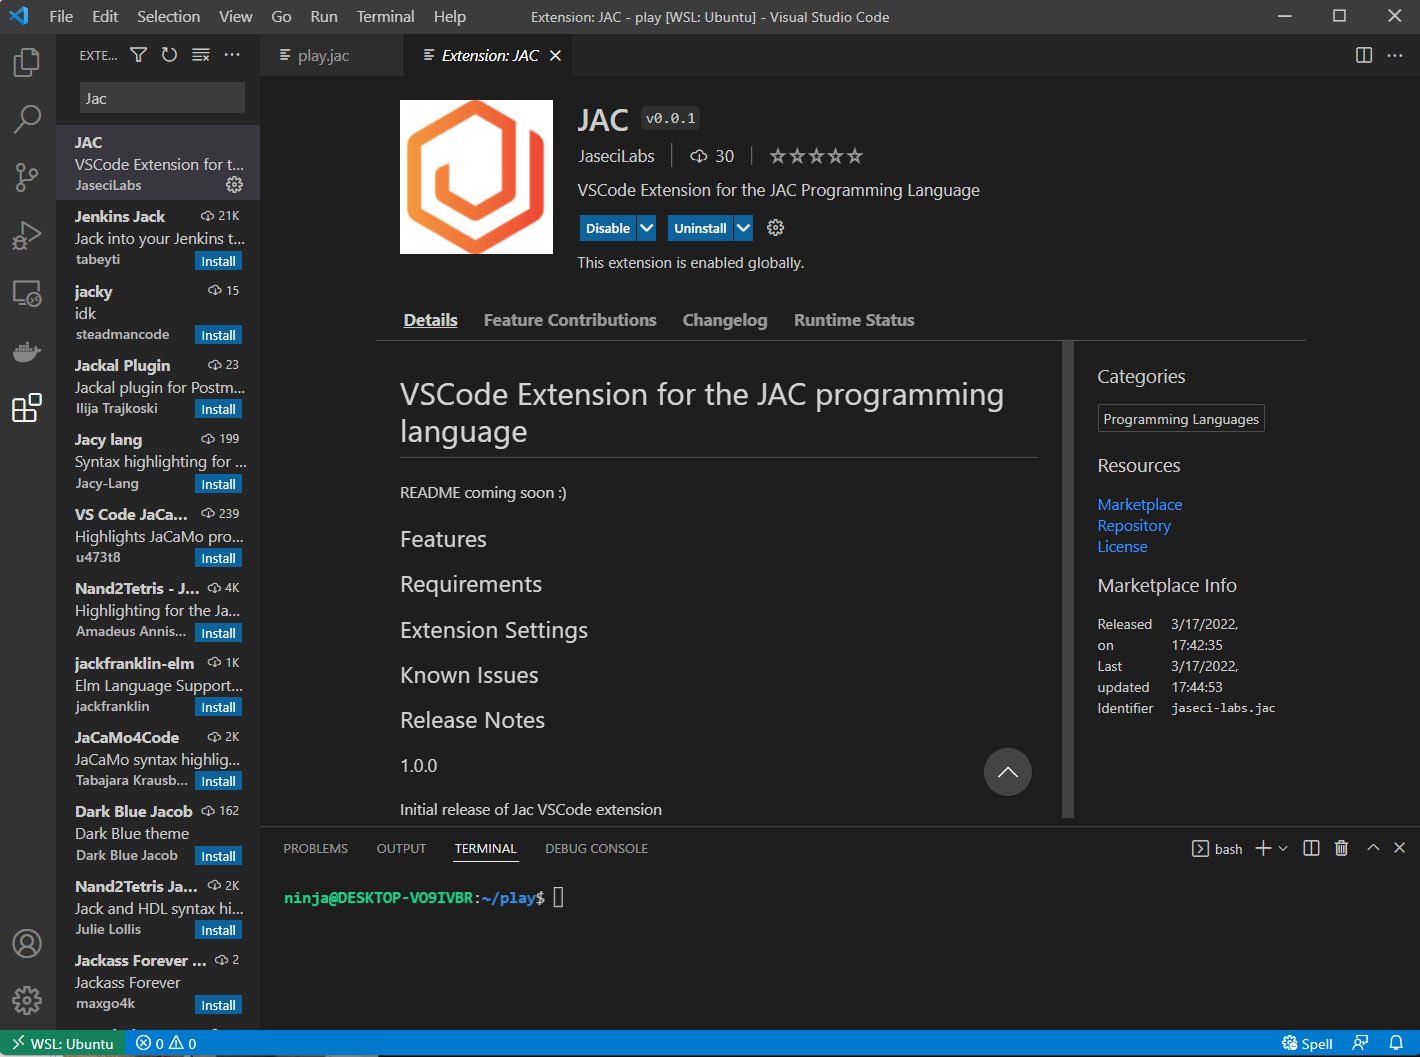
\includegraphics[width=.7\linewidth]{assets/images/vscode_jac_plugin.png}
    \caption[]{The Wonderful Jac Language extension in VSCode.}
    \label{fig:vscode_jac}
\end{figure}

\par
In VSCode, you can search for and install the Jac language extensions as per Figure~\ref{fig:vscode_jac}. As you can see, at the time I clipped this image, its quite new and doesn't really have a readme. You won't need one, it just provides syntax highlighting for \texttt{.jac} files at the moment. But it makes Jac code look beautiful, so it's a must have. 

\section{Coding Jac}